% Options for packages loaded elsewhere
\PassOptionsToPackage{unicode}{hyperref}
\PassOptionsToPackage{hyphens}{url}
%
\documentclass[
]{article}
\usepackage{amsmath,amssymb}
\usepackage{lmodern}
\usepackage{iftex}
\ifPDFTeX
  \usepackage[T1]{fontenc}
  \usepackage[utf8]{inputenc}
  \usepackage{textcomp} % provide euro and other symbols
\else % if luatex or xetex
  \usepackage{unicode-math}
  \defaultfontfeatures{Scale=MatchLowercase}
  \defaultfontfeatures[\rmfamily]{Ligatures=TeX,Scale=1}
\fi
% Use upquote if available, for straight quotes in verbatim environments
\IfFileExists{upquote.sty}{\usepackage{upquote}}{}
\IfFileExists{microtype.sty}{% use microtype if available
  \usepackage[]{microtype}
  \UseMicrotypeSet[protrusion]{basicmath} % disable protrusion for tt fonts
}{}
\makeatletter
\@ifundefined{KOMAClassName}{% if non-KOMA class
  \IfFileExists{parskip.sty}{%
    \usepackage{parskip}
  }{% else
    \setlength{\parindent}{0pt}
    \setlength{\parskip}{6pt plus 2pt minus 1pt}}
}{% if KOMA class
  \KOMAoptions{parskip=half}}
\makeatother
\usepackage{xcolor}
\IfFileExists{xurl.sty}{\usepackage{xurl}}{} % add URL line breaks if available
\IfFileExists{bookmark.sty}{\usepackage{bookmark}}{\usepackage{hyperref}}
\hypersetup{
  pdftitle={ADULT CENSUS ANALYSIS},
  pdfauthor={Fabrizio Niro 5106988},
  hidelinks,
  pdfcreator={LaTeX via pandoc}}
\urlstyle{same} % disable monospaced font for URLs
\usepackage[margin=1in]{geometry}
\usepackage{color}
\usepackage{fancyvrb}
\newcommand{\VerbBar}{|}
\newcommand{\VERB}{\Verb[commandchars=\\\{\}]}
\DefineVerbatimEnvironment{Highlighting}{Verbatim}{commandchars=\\\{\}}
% Add ',fontsize=\small' for more characters per line
\usepackage{framed}
\definecolor{shadecolor}{RGB}{248,248,248}
\newenvironment{Shaded}{\begin{snugshade}}{\end{snugshade}}
\newcommand{\AlertTok}[1]{\textcolor[rgb]{0.94,0.16,0.16}{#1}}
\newcommand{\AnnotationTok}[1]{\textcolor[rgb]{0.56,0.35,0.01}{\textbf{\textit{#1}}}}
\newcommand{\AttributeTok}[1]{\textcolor[rgb]{0.77,0.63,0.00}{#1}}
\newcommand{\BaseNTok}[1]{\textcolor[rgb]{0.00,0.00,0.81}{#1}}
\newcommand{\BuiltInTok}[1]{#1}
\newcommand{\CharTok}[1]{\textcolor[rgb]{0.31,0.60,0.02}{#1}}
\newcommand{\CommentTok}[1]{\textcolor[rgb]{0.56,0.35,0.01}{\textit{#1}}}
\newcommand{\CommentVarTok}[1]{\textcolor[rgb]{0.56,0.35,0.01}{\textbf{\textit{#1}}}}
\newcommand{\ConstantTok}[1]{\textcolor[rgb]{0.00,0.00,0.00}{#1}}
\newcommand{\ControlFlowTok}[1]{\textcolor[rgb]{0.13,0.29,0.53}{\textbf{#1}}}
\newcommand{\DataTypeTok}[1]{\textcolor[rgb]{0.13,0.29,0.53}{#1}}
\newcommand{\DecValTok}[1]{\textcolor[rgb]{0.00,0.00,0.81}{#1}}
\newcommand{\DocumentationTok}[1]{\textcolor[rgb]{0.56,0.35,0.01}{\textbf{\textit{#1}}}}
\newcommand{\ErrorTok}[1]{\textcolor[rgb]{0.64,0.00,0.00}{\textbf{#1}}}
\newcommand{\ExtensionTok}[1]{#1}
\newcommand{\FloatTok}[1]{\textcolor[rgb]{0.00,0.00,0.81}{#1}}
\newcommand{\FunctionTok}[1]{\textcolor[rgb]{0.00,0.00,0.00}{#1}}
\newcommand{\ImportTok}[1]{#1}
\newcommand{\InformationTok}[1]{\textcolor[rgb]{0.56,0.35,0.01}{\textbf{\textit{#1}}}}
\newcommand{\KeywordTok}[1]{\textcolor[rgb]{0.13,0.29,0.53}{\textbf{#1}}}
\newcommand{\NormalTok}[1]{#1}
\newcommand{\OperatorTok}[1]{\textcolor[rgb]{0.81,0.36,0.00}{\textbf{#1}}}
\newcommand{\OtherTok}[1]{\textcolor[rgb]{0.56,0.35,0.01}{#1}}
\newcommand{\PreprocessorTok}[1]{\textcolor[rgb]{0.56,0.35,0.01}{\textit{#1}}}
\newcommand{\RegionMarkerTok}[1]{#1}
\newcommand{\SpecialCharTok}[1]{\textcolor[rgb]{0.00,0.00,0.00}{#1}}
\newcommand{\SpecialStringTok}[1]{\textcolor[rgb]{0.31,0.60,0.02}{#1}}
\newcommand{\StringTok}[1]{\textcolor[rgb]{0.31,0.60,0.02}{#1}}
\newcommand{\VariableTok}[1]{\textcolor[rgb]{0.00,0.00,0.00}{#1}}
\newcommand{\VerbatimStringTok}[1]{\textcolor[rgb]{0.31,0.60,0.02}{#1}}
\newcommand{\WarningTok}[1]{\textcolor[rgb]{0.56,0.35,0.01}{\textbf{\textit{#1}}}}
\usepackage{graphicx}
\makeatletter
\def\maxwidth{\ifdim\Gin@nat@width>\linewidth\linewidth\else\Gin@nat@width\fi}
\def\maxheight{\ifdim\Gin@nat@height>\textheight\textheight\else\Gin@nat@height\fi}
\makeatother
% Scale images if necessary, so that they will not overflow the page
% margins by default, and it is still possible to overwrite the defaults
% using explicit options in \includegraphics[width, height, ...]{}
\setkeys{Gin}{width=\maxwidth,height=\maxheight,keepaspectratio}
% Set default figure placement to htbp
\makeatletter
\def\fps@figure{htbp}
\makeatother
\setlength{\emergencystretch}{3em} % prevent overfull lines
\providecommand{\tightlist}{%
  \setlength{\itemsep}{0pt}\setlength{\parskip}{0pt}}
\setcounter{secnumdepth}{-\maxdimen} % remove section numbering
\ifLuaTeX
  \usepackage{selnolig}  % disable illegal ligatures
\fi

\title{ADULT CENSUS ANALYSIS}
\usepackage{etoolbox}
\makeatletter
\providecommand{\subtitle}[1]{% add subtitle to \maketitle
  \apptocmd{\@title}{\par {\large #1 \par}}{}{}
}
\makeatother
\subtitle{Bayesian Modelling}
\author{Fabrizio Niro 5106988}
\date{18/07/2022}

\begin{document}
\maketitle

\hypertarget{introduction}{%
\subsection{Introduction}\label{introduction}}

The dataset object of this analysis is ``Adult Census'' dataset. It is
also known as ``Adult'' dataset. It has been donated to UCI from Ronny
Kohavi and Barry Becker in 1996. The data has been extracted by Barry
Becker from the 1994 Census database. The dataset used in this analysis
has more than 30k observations and 9 variables had been selected.

The aim of this project is to build a Bayesian Model for predicting the
probability that a person has an income greater than 50K dollars in a
year.

In order to do this, we will implement a Logistic Regression to model
the binary response (0 = ``income'' \textless=50K, 1 = ``income''
\textgreater{} 50K) and a Multivariate Gaussian Copula Model, which will
accomplish the task of explaining the dependencies between the
covariates.

\hypertarget{dataset-description}{%
\subsection{Dataset description}\label{dataset-description}}

The variable \textbf{Income} (binary) depends on the data through 8
predictors:

\begin{itemize}
\item
  \textbf{Sex}: Factor variable with levels ``Female'' and ``Male''
\item
  \textbf{Age}: Integer variable containing the age of the person
\item
  \textbf{Race}: Factor variable with levels ``Black'', ``White'',
  ``Other''
\item
  \textbf{Native\_region}: Factor variable which contains the region of
  birth of the person, it has levels: ``United States'',
  ``Central-America'', ``South-America'', ``Europe-West'',
  ``Europe-East'', ``Asia-West'', ``Asia-East''
\item
  \textbf{Education\_num}: Integer variable which contains the total
  amount of education years of the person
\item
  \textbf{Workclass}: Factor variable which describes the sector of
  working, it has levels: ``Self-employed'', ``Private'',
  ``Government'', ``Other''
\item
  \textbf{Hours\_per\_week}: Integer variable related to the total
  working hours per week
\item
  \textbf{Capital\_gain}: Integer variable which reporting the total
  capital gain of the person in a year. It can take negative values for
  capital losses.
\end{itemize}

\begin{verbatim}
##      sex age  race   native_region education_num     workclass hours_per_week
## 1   Male  39 White   United-States            13    Government             40
## 2   Male  50 White   United-States            13 Self-employed             13
## 3   Male  38 White   United-States             9       Private             40
## 4   Male  53 Black   United-States             7       Private             40
## 5 Female  28 Black Central-America            13       Private             40
## 6 Female  37 White   United-States            14       Private             40
##   capital_gain income
## 1         2174      0
## 2            0      0
## 3            0      0
## 4            0      0
## 5            0      0
## 6            0      0
\end{verbatim}

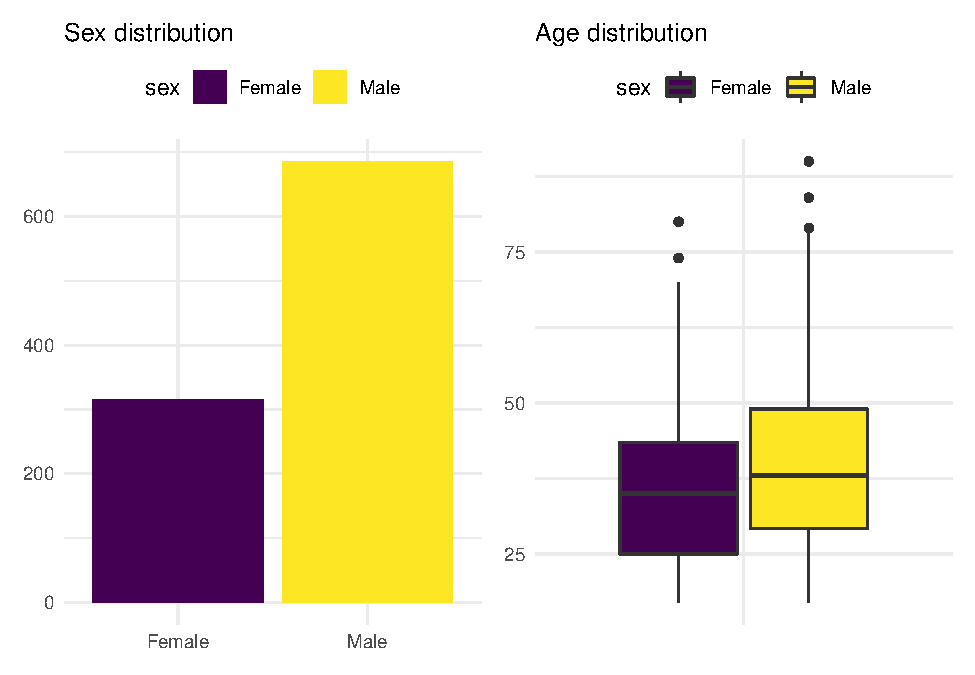
\includegraphics{bmp_main_files/figure-latex/sex_age plots-1.pdf}

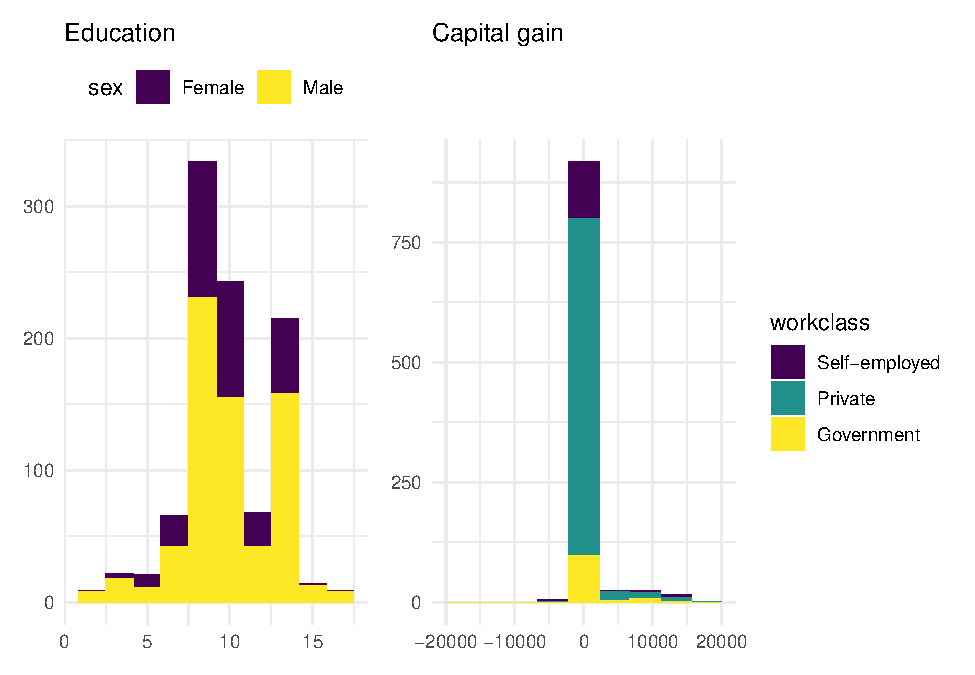
\includegraphics{bmp_main_files/figure-latex/edu_cap plots-1.pdf}

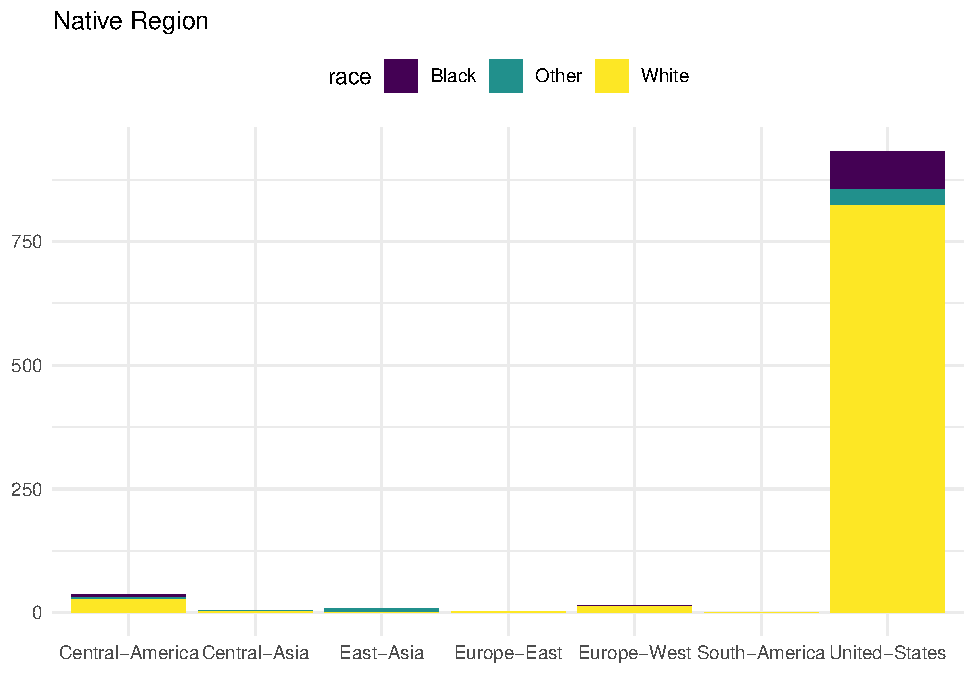
\includegraphics{bmp_main_files/figure-latex/native plot-1.pdf} \#\#
Model \{.tabset\}

\hypertarget{logistic-regression-with-spike-and-slab-prior}{%
\subsubsection{Logistic regression with Spike and Slab
prior}\label{logistic-regression-with-spike-and-slab-prior}}

In order to model the effects of the predictors on the response, we will
implement a \textbf{General Linear Model for binary data}, with
\textbf{logistic link function}. Furthermore, we will use a
\textbf{``Spike and Slab'' Prior} in order to perform model selection,
as in the case of GLMs it is not possible to to compute the
\textbf{posterior model probability}, which implicitly performs
predictor selection.

Assume the response variable \(Y\) is binary, \(Y \in {0,1}\)

\[Y_i | \pi_i \sim Bern(\pi_i) \qquad i=1,...,n\]

\[\pi_i = h(\beta^T x_i)\] where \(h()\) is an Inverse-Link function
which guarantees that \(E(Y|.) \in \{0,1\}\)

for the cas eof logistic regression:

\[logit(\pi_i) = log \bigg( \frac{\pi_i}{1 - \pi_i} \bigg) = \eta = \beta^Tx_i\]
the logistic function is then found as:

\[\frac{\pi_i}{1 - \pi_i} = \eta\]

\[\pi_i = \frac{\exp(\beta^Tx_i)}{1 + \exp(\beta^Tx_i)}\]

The likelihood is:

\[p(y | \beta) = \prod_{i=1}^n p(y_i | \pi_i)   = \prod_{i=1}^n \pi^{y_i}(1 - \pi_i)^{1-y_i} = \prod_{i=1}^n h(\beta^Tx_i)^y_i (1-h(\beta^Tx_i))^{1-y_I}\]

While the Prior on \(\beta = (\beta_1,...,\beta_p)^T\) is:

\[\beta_j \sim N(\beta_{0j}, \sigma^2_{0j})\]

\[p(\beta) = \prod_{j=1}^p dN(\beta_j | \beta_{0j}, \sigma^2_{0j})\]

Which is not conjugate to the model. The following posterior
distribution should be therefore approximated using a Metropolis
Hastings algorithm.

\[p(\beta | y) \propto p(y | \beta)p(\beta)\]

\hypertarget{spike-and-slab-prior}{%
\subparagraph{Spike and Slab Prior}\label{spike-and-slab-prior}}

Consider a GLM of the form

\[E(Y|x) = h(\beta_1 X_1 + ... + \beta_pX_p)\]

we introduce a \((p,1)\) binary vector
\(\gamma = (\gamma_1,...,\gamma_p)^T\) such that

\[\gamma_j = \begin{cases} 1 & \mbox{if} \qquad X_j \quad \mbox{is included in the model}\\ 0 & \mbox{if} \qquad X_j \quad \mbox{is not included in the model} \end{cases}\]

so that \(\gamma_j\) ``controls'' the inclusion of X\_j among the
predictors.

We treat \(\gamma\) as a parameter and do posterior inference on it We
then write:

\[E(Y|x) = h(\gamma_1\beta_1 X_1 + ... + \gamma_p\beta_pX_p)\] So we now
need to assign priors both to \(\gamma = (\gamma_1,...,\gamma_p)^T\) and
\(\beta = (\beta_1,...,\beta_p)^T\)

that are:

\[\gamma_j \sim Bern(w) \qquad \beta_j \sim N(\beta_{0j},\sigma^2_{0j})\]

\hypertarget{implementation-of-metropolis-hastings-algorithm-using-jags}{%
\subparagraph{Implementation of Metropolis Hastings algorithm using
JAGS}\label{implementation-of-metropolis-hastings-algorithm-using-jags}}

The Metropolis Hastings algorithm is a generalization of Gibbs and
Metropolis algorithm, general methods used to approximate functions or
distribution \(f(x)\). In the case of Bayesian statistics they are
widely implemented to approximate posterior distributions.

In this case we need to approximate the vector of parameter
\(\beta_j = (\beta_\,...,\beta_p)\) starting from initial values
\(\beta_1^{(1)},...,\beta_p^{(1)}\)

Given \(S = 5000\) the number of MCMC iterations,

For \(s = 1,...,S\)\\
\hspace*{0.333em}\hspace*{0.333em}\hspace*{0.333em}For \(j = 1,...,p\)

\begin{enumerate}
\def\labelenumi{\arabic{enumi}.}
\tightlist
\item
  Propose \(\beta^*_j \sim q(\beta_j|\beta_j^{(s)})\) from a Normal
  \(dN(\beta_j^*| \beta_j^{(s)},\delta^2_j)\) centered at current value
  \(\beta_j^{(s)}\) (mean) and with fixed \(\delta^2_j\) (variance)
\end{enumerate}

\begin{enumerate}
\def\labelenumi{\arabic{enumi}.}
\setcounter{enumi}{1}
\tightlist
\item
  Compute
  \(r_j = \frac{p(\beta_j^*,\beta_{-j}^{(s)} | y)}{p(\beta_j^s,\beta_{-j}^{(s)} | y)} \frac{q(\beta_j^{(s)} | \beta_j^*)}{q(\beta_j^{(*)} | \beta_j^s)}\)
  which is the ratio of posteriors, that does not require the
  computation of \(p(y)\), the marginal likelihood, which is not
  available analytically.
\end{enumerate}

\begin{enumerate}
\def\labelenumi{\arabic{enumi}.}
\setcounter{enumi}{2}
\tightlist
\item
  Set
  \(\beta_j^{(s+1)} = \begin{cases} \beta_j^* & \mbox{with probability} \quad min\{r_j,1\} \\ \beta_j^{(s)} & \mbox{with probability} \quad 1 - min\{r_j,1\} \end{cases}\)
\end{enumerate}

Finally, we obtain the dependent sequence

\(\beta = \{\beta^{(1)},...,\beta^{(S)}\}\) with
\(\beta^{(s)} = \{\beta^{(s)}_1,...,\beta^{(S)}_p\}\)

In order to implement it, the first step is expanding factor variables
into dummies and adding the Intercept

\begin{verbatim}
##   (Intercept) sexMale age raceOther raceWhite native_regionCentral-Asia
## 1           1       1  44         0         1                         0
## 2           1       1  55         0         1                         0
## 3           1       1  34         0         1                         0
## 4           1       1  33         0         1                         0
## 5           1       1  36         0         1                         0
## 6           1       0  25         0         1                         0
##   native_regionEast-Asia native_regionEurope-East native_regionEurope-West
## 1                      0                        0                        0
## 2                      0                        0                        0
## 3                      0                        0                        0
## 4                      0                        0                        0
## 5                      0                        0                        0
## 6                      0                        0                        0
##   native_regionSouth-America native_regionUnited-States education_num
## 1                          0                          1            13
## 2                          0                          1             9
## 3                          0                          1            10
## 4                          0                          1            14
## 5                          0                          1            13
## 6                          0                          1             9
##   workclassPrivate workclassGovernment workclassOther hours_per_week
## 1                1                   0              0             12
## 2                1                   0              0             40
## 3                1                   0              0             40
## 4                1                   0              0             40
## 5                1                   0              0             55
## 6                1                   0              0             40
##   capital_gain
## 1            0
## 2            0
## 3            0
## 4            0
## 5            0
## 6            0
\end{verbatim}

\begin{Shaded}
\begin{Highlighting}[]
\NormalTok{jags\_data }\OtherTok{=} \FunctionTok{with}\NormalTok{(X, }\FunctionTok{list}\NormalTok{(}\AttributeTok{y =}\NormalTok{ y, }\AttributeTok{X =}\NormalTok{ X, }\AttributeTok{n =} \FunctionTok{length}\NormalTok{(y), }\AttributeTok{p =} \FunctionTok{ncol}\NormalTok{(X)))}
\end{Highlighting}
\end{Shaded}

\begin{Shaded}
\begin{Highlighting}[]
\NormalTok{logistic\_regr\_jags }\OtherTok{=} \ControlFlowTok{function}\NormalTok{()\{}
  
  \DocumentationTok{\#\#\#\#\#\#\#\#\#\#\#\#\#\#}
  \CommentTok{\# Likelihood \#}
  \DocumentationTok{\#\#\#\#\#\#\#\#\#\#\#\#\#\#}
  
  \ControlFlowTok{for}\NormalTok{(i }\ControlFlowTok{in} \DecValTok{1}\SpecialCharTok{:}\NormalTok{n)\{}
    
\NormalTok{    y[i] }\SpecialCharTok{\textasciitilde{}} \FunctionTok{dbern}\NormalTok{(pi[i])}
    
    \FunctionTok{logit}\NormalTok{(pi[i]) }\OtherTok{=}\NormalTok{ (gamma }\SpecialCharTok{*}\NormalTok{ beta) }\SpecialCharTok{\%*\%}\NormalTok{ X [i,]}
\NormalTok{  \}}
  
  \DocumentationTok{\#\#\#\#\#\#\#\#\#\#}
  \CommentTok{\# Priors \#}
  \DocumentationTok{\#\#\#\#\#\#\#\#\#\#}
  
  \ControlFlowTok{for}\NormalTok{(j }\ControlFlowTok{in} \DecValTok{1}\SpecialCharTok{:}\NormalTok{p)\{}

\NormalTok{    beta[j] }\SpecialCharTok{\textasciitilde{}} \FunctionTok{dnorm}\NormalTok{(}\DecValTok{0}\NormalTok{, }\FloatTok{0.01}\NormalTok{) }
\NormalTok{  \}}
  
  \ControlFlowTok{for}\NormalTok{(j }\ControlFlowTok{in} \DecValTok{1}\SpecialCharTok{:}\NormalTok{p)\{}

\NormalTok{    gamma[j] }\SpecialCharTok{\textasciitilde{}} \FunctionTok{dbern}\NormalTok{(w) }
\NormalTok{  \}}
  
\NormalTok{  w }\SpecialCharTok{\textasciitilde{}} \FunctionTok{dbeta}\NormalTok{(}\DecValTok{1}\NormalTok{,}\DecValTok{1}\NormalTok{)}
\NormalTok{\}}
\end{Highlighting}
\end{Shaded}

\begin{Shaded}
\begin{Highlighting}[]
\NormalTok{init\_values }\OtherTok{=} \ControlFlowTok{function}\NormalTok{()\{}
  
  \FunctionTok{list}\NormalTok{(}\AttributeTok{beta =} \FunctionTok{rep}\NormalTok{(}\DecValTok{0}\NormalTok{, }\FunctionTok{ncol}\NormalTok{(X)), }\AttributeTok{gamma =} \FunctionTok{rep}\NormalTok{(}\DecValTok{1}\NormalTok{, }\FunctionTok{ncol}\NormalTok{(X)))}
  
\NormalTok{\}}

\NormalTok{params }\OtherTok{=} \FunctionTok{c}\NormalTok{(}\StringTok{"beta"}\NormalTok{, }\StringTok{"gamma"}\NormalTok{)}
\end{Highlighting}
\end{Shaded}

\begin{Shaded}
\begin{Highlighting}[]
\NormalTok{jags\_post.mcmc }\OtherTok{\textless{}{-}} \FunctionTok{as.mcmc}\NormalTok{(jags\_posterior)}

\NormalTok{S }\OtherTok{\textless{}{-}} \FunctionTok{ggs}\NormalTok{(jags\_post.mcmc)}


\CommentTok{\# ggmcmc(S)}
\end{Highlighting}
\end{Shaded}

\begin{Shaded}
\begin{Highlighting}[]
\NormalTok{out }\OtherTok{=}\NormalTok{ jags\_posterior}\SpecialCharTok{$}\NormalTok{BUGSoutput}

\DocumentationTok{\#\# Extract samples from the posterior of beta and gamma}

\NormalTok{beta\_post  }\OtherTok{=}\NormalTok{ out}\SpecialCharTok{$}\NormalTok{sims.list}\SpecialCharTok{$}\NormalTok{beta}
\NormalTok{gamma\_post }\OtherTok{=}\NormalTok{ out}\SpecialCharTok{$}\NormalTok{sims.list}\SpecialCharTok{$}\NormalTok{gamma}

\FunctionTok{dim}\NormalTok{(gamma\_post)}
\end{Highlighting}
\end{Shaded}

\begin{verbatim}
## [1] 2000   17
\end{verbatim}

\begin{Shaded}
\begin{Highlighting}[]
\NormalTok{S }\OtherTok{=} \FunctionTok{nrow}\NormalTok{(gamma\_post)}

\DocumentationTok{\#\# Estimate the posterior probability of inclusion of each predictor Xj}
\DocumentationTok{\#\# i.e. proportion of times gammaj = 1}

\NormalTok{prob\_inclusion }\OtherTok{=} \FunctionTok{colMeans}\NormalTok{(gamma\_post)}
\end{Highlighting}
\end{Shaded}

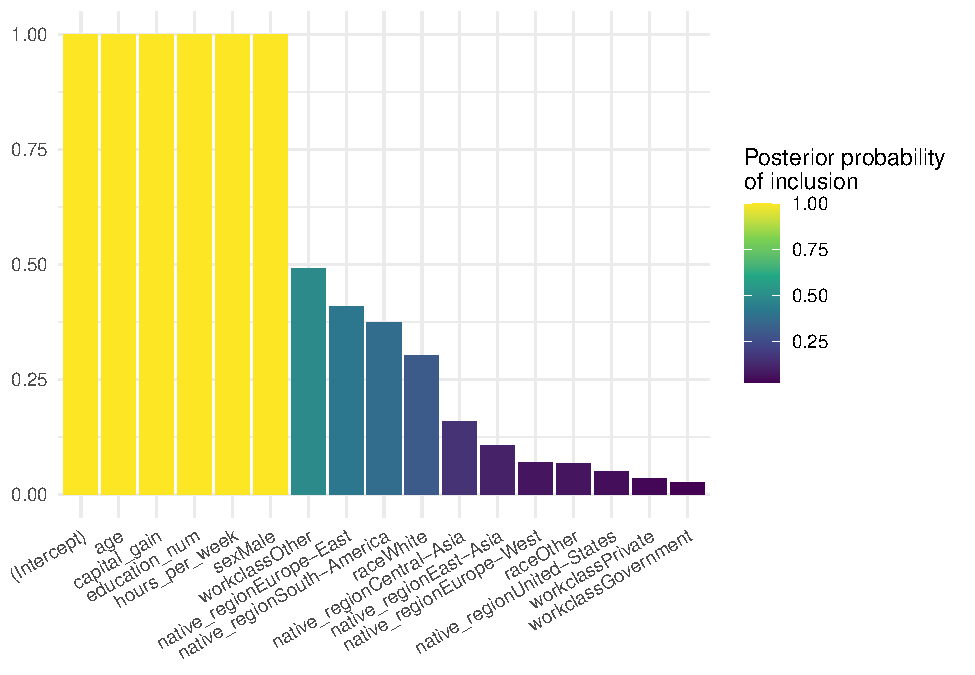
\includegraphics{bmp_main_files/figure-latex/unnamed-chunk-6-1.pdf}

\begin{Shaded}
\begin{Highlighting}[]
\NormalTok{x.star }\OtherTok{\textless{}{-}} \FunctionTok{as.numeric}\NormalTok{(X.t[}\DecValTok{3}\NormalTok{,])}

\NormalTok{S }\OtherTok{\textless{}{-}} \FunctionTok{nrow}\NormalTok{(gamma\_post)}
\NormalTok{eta }\OtherTok{\textless{}{-}} \FunctionTok{numeric}\NormalTok{(S)}

\ControlFlowTok{for}\NormalTok{(s }\ControlFlowTok{in} \DecValTok{1}\SpecialCharTok{:}\NormalTok{S)\{}
  
\NormalTok{  eta[s] }\OtherTok{\textless{}{-}}\NormalTok{ (gamma\_post[s,]}\SpecialCharTok{*}\NormalTok{beta\_post[s,]) }\SpecialCharTok{\%*\%}\NormalTok{ x.star}
  
\NormalTok{\}}

\NormalTok{pi.star }\OtherTok{=} \FunctionTok{exp}\NormalTok{(eta)}\SpecialCharTok{/}\NormalTok{(}\DecValTok{1} \SpecialCharTok{+} \FunctionTok{exp}\NormalTok{(eta))}

\DocumentationTok{\#\# Approximate predictive distribution is}
\FunctionTok{hist}\NormalTok{(pi.star)}
\end{Highlighting}
\end{Shaded}

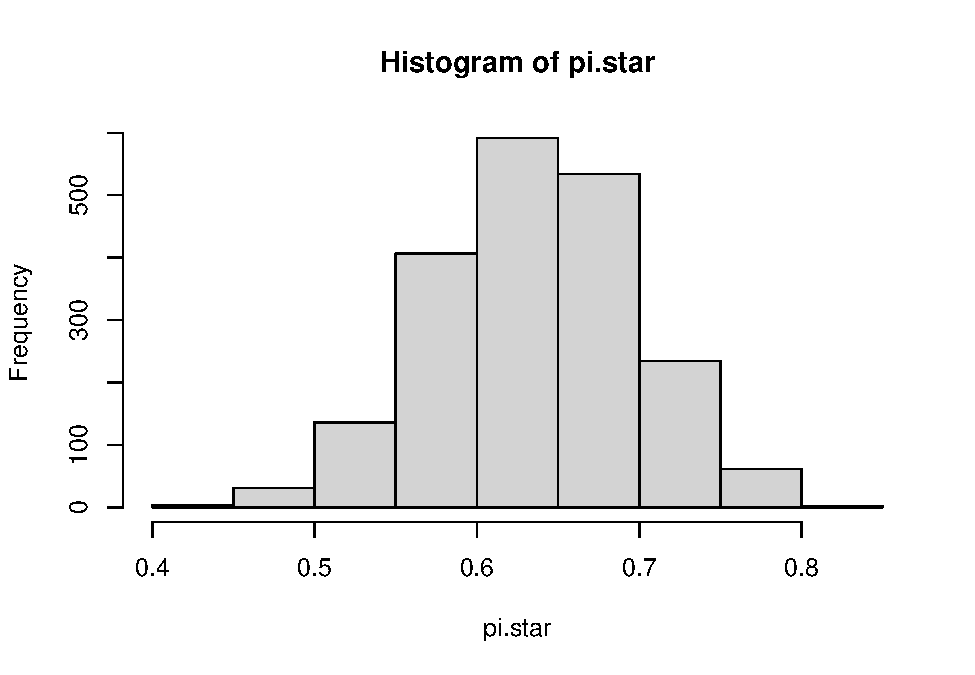
\includegraphics{bmp_main_files/figure-latex/unnamed-chunk-7-1.pdf}

\begin{Shaded}
\begin{Highlighting}[]
\NormalTok{pi.star }\OtherTok{\textless{}{-}} \FunctionTok{as.data.frame}\NormalTok{(pi.star)}

\FunctionTok{ggplot}\NormalTok{(pi.star, }\FunctionTok{aes}\NormalTok{(}\AttributeTok{x =}\NormalTok{ pi.star, }\AttributeTok{fill=}\NormalTok{pi.star)) }\SpecialCharTok{+} \FunctionTok{geom\_histogram}\NormalTok{() }\SpecialCharTok{+} \FunctionTok{scale\_fill\_viridis\_c}\NormalTok{() }\SpecialCharTok{+} \FunctionTok{theme\_minimal}\NormalTok{()}
\end{Highlighting}
\end{Shaded}

\begin{verbatim}
## `stat_bin()` using `bins = 30`. Pick better value with `binwidth`.
\end{verbatim}

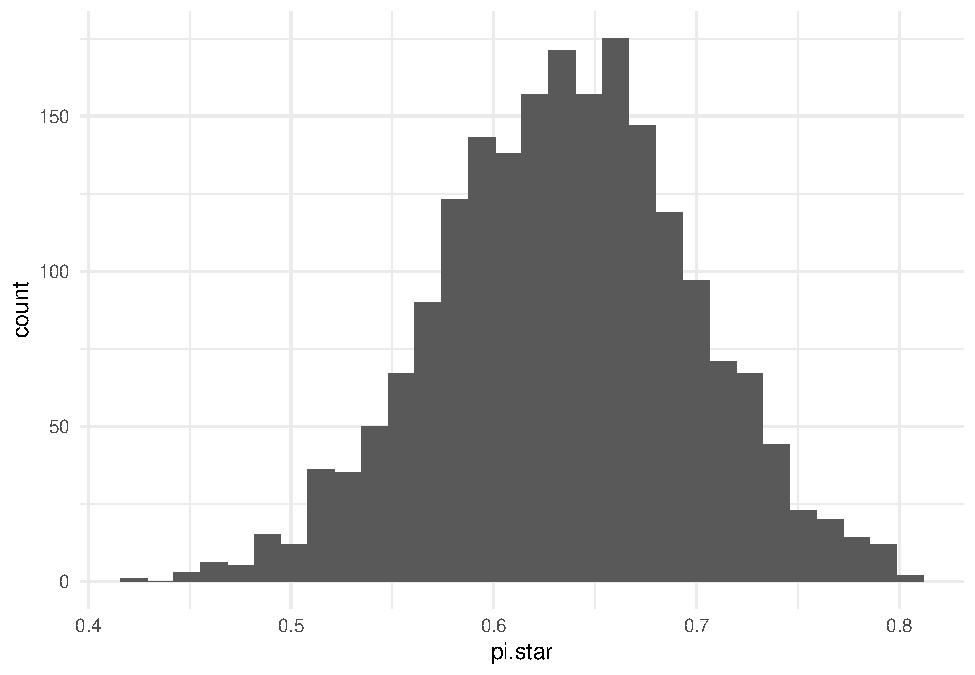
\includegraphics{bmp_main_files/figure-latex/unnamed-chunk-7-2.pdf}

\begin{Shaded}
\begin{Highlighting}[]
\FunctionTok{boxplot}\NormalTok{(pi.star, }\AttributeTok{main =} \StringTok{""}\NormalTok{, }\AttributeTok{ylim =} \FunctionTok{c}\NormalTok{(}\DecValTok{0}\NormalTok{,}\DecValTok{1}\NormalTok{), }\AttributeTok{xlab =} \FunctionTok{expression}\NormalTok{(pi), }\AttributeTok{horizontal =} \ConstantTok{TRUE}\NormalTok{,}
        \AttributeTok{border =} \FunctionTok{c}\NormalTok{(}\StringTok{"blue"}\NormalTok{))}
\end{Highlighting}
\end{Shaded}

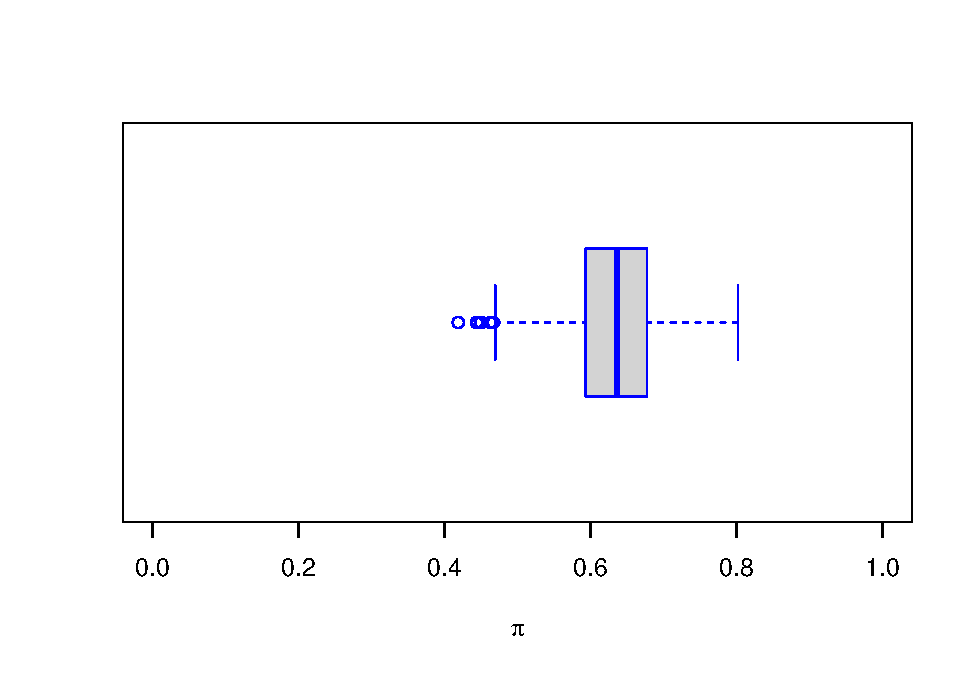
\includegraphics{bmp_main_files/figure-latex/unnamed-chunk-8-1.pdf}

\begin{Shaded}
\begin{Highlighting}[]
\FunctionTok{ggplot}\NormalTok{(pi.star, }\FunctionTok{aes}\NormalTok{(}\AttributeTok{x =}\NormalTok{ pi.star)) }\SpecialCharTok{+} \FunctionTok{geom\_boxplot}\NormalTok{() }\SpecialCharTok{+} \FunctionTok{theme\_minimal}\NormalTok{() }\SpecialCharTok{+} \FunctionTok{scale\_fill\_viridis\_c}\NormalTok{()}
\end{Highlighting}
\end{Shaded}

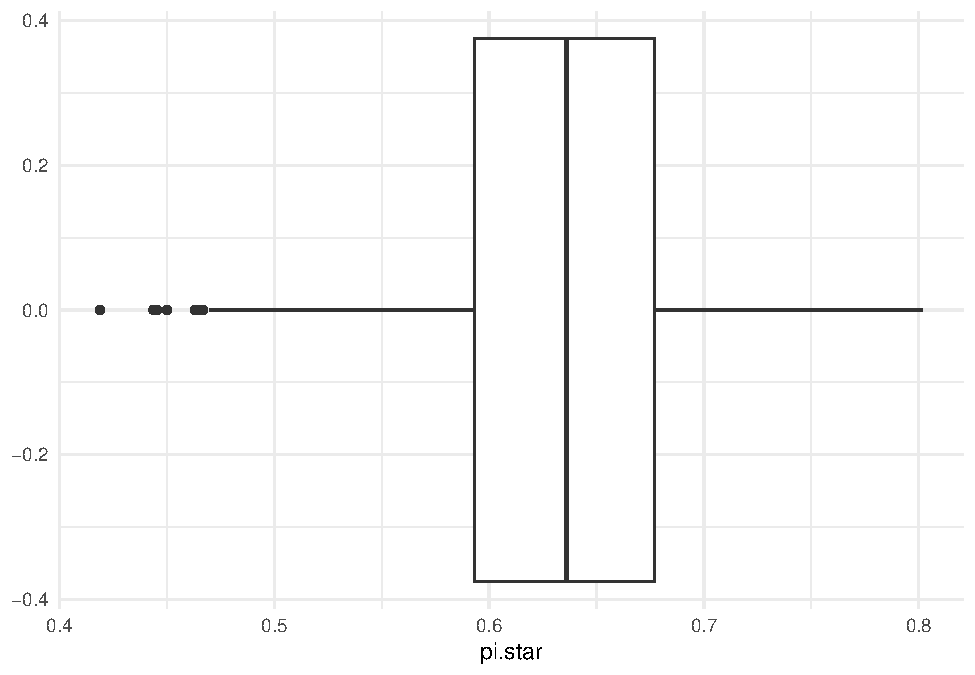
\includegraphics{bmp_main_files/figure-latex/unnamed-chunk-8-2.pdf}

\begin{Shaded}
\begin{Highlighting}[]
\DocumentationTok{\#\# 95\%  credible intervals}
\NormalTok{cred.int }\OtherTok{\textless{}{-}} \FunctionTok{t}\NormalTok{(}\FunctionTok{apply}\NormalTok{(beta\_post, }\DecValTok{2}\NormalTok{, quantile, }\FunctionTok{c}\NormalTok{(.}\DecValTok{025}\NormalTok{, .}\DecValTok{975}\NormalTok{)))}

\DocumentationTok{\#\# probs of predictors having a positive effect on the logit}
\FunctionTok{colMeans}\NormalTok{(}\FunctionTok{apply}\NormalTok{(beta\_post, }\DecValTok{2}\NormalTok{, }\ControlFlowTok{function}\NormalTok{(x) x }\SpecialCharTok{\textgreater{}} \DecValTok{0}\NormalTok{))}
\end{Highlighting}
\end{Shaded}

\begin{verbatim}
##  [1] 0.0000 1.0000 1.0000 0.4890 0.6445 0.4380 0.5030 0.3310 0.5040 0.3830
## [11] 0.5000 1.0000 0.5095 0.4845 0.4940 1.0000 1.0000
\end{verbatim}

\begin{Shaded}
\begin{Highlighting}[]
\CommentTok{\#par(mar = c(8,5,1,1))}
\CommentTok{\#}
\CommentTok{\#boxplot(beta\_post, outline = F, ylim = c({-}30,30), ylab = expression(beta), xlab = \#names(beta\_post), cex.axis = 0.7, las = 2)}
\CommentTok{\#abline(h = 0, col = "blue", lty = "dashed")}
\CommentTok{\#out\_glm = summary(glm(y \textasciitilde{} X {-} 1, family = "binomial"))}
\CommentTok{\#points(out\_glm$coefficients[,1], col = "blue", pch = 16)}
\end{Highlighting}
\end{Shaded}

\hypertarget{multivariate-gaussian-copula-model}{%
\subsubsection{Multivariate Gaussian copula
model}\label{multivariate-gaussian-copula-model}}

\begin{Shaded}
\begin{Highlighting}[]
\CommentTok{\#source("sbgcop\_modified.R")}
\CommentTok{\#}
\CommentTok{\#fit \textless{}{-} sbgcop.mcmc.bis(Y=X)}
\CommentTok{\#}
\CommentTok{\#summary(fit)}
\end{Highlighting}
\end{Shaded}


\end{document}
